Optimizing hyperparameters for this section was trivial due to relatively low performance expectations.
The training of the following two networks was more a sanity check than anything else.
As such, we simply present the architectures found that satisfied the specs and plots of our results.
\begin{itemize}[topsep=-15pt, noitemsep, nolistsep]
  
  \item \textbf{Overfitting a net}\\
    Architecture: 1 hidden layer with 50 hidden units.\\
    Hyperparameters: sgd update rule, 5e-4 learning rate, 0.85 learning rate decay, 20 epochs and a batch size of 5.
    \include*{../nets/overfit_net/info}

    \begin{figure}[!ht]
        \centering
        {{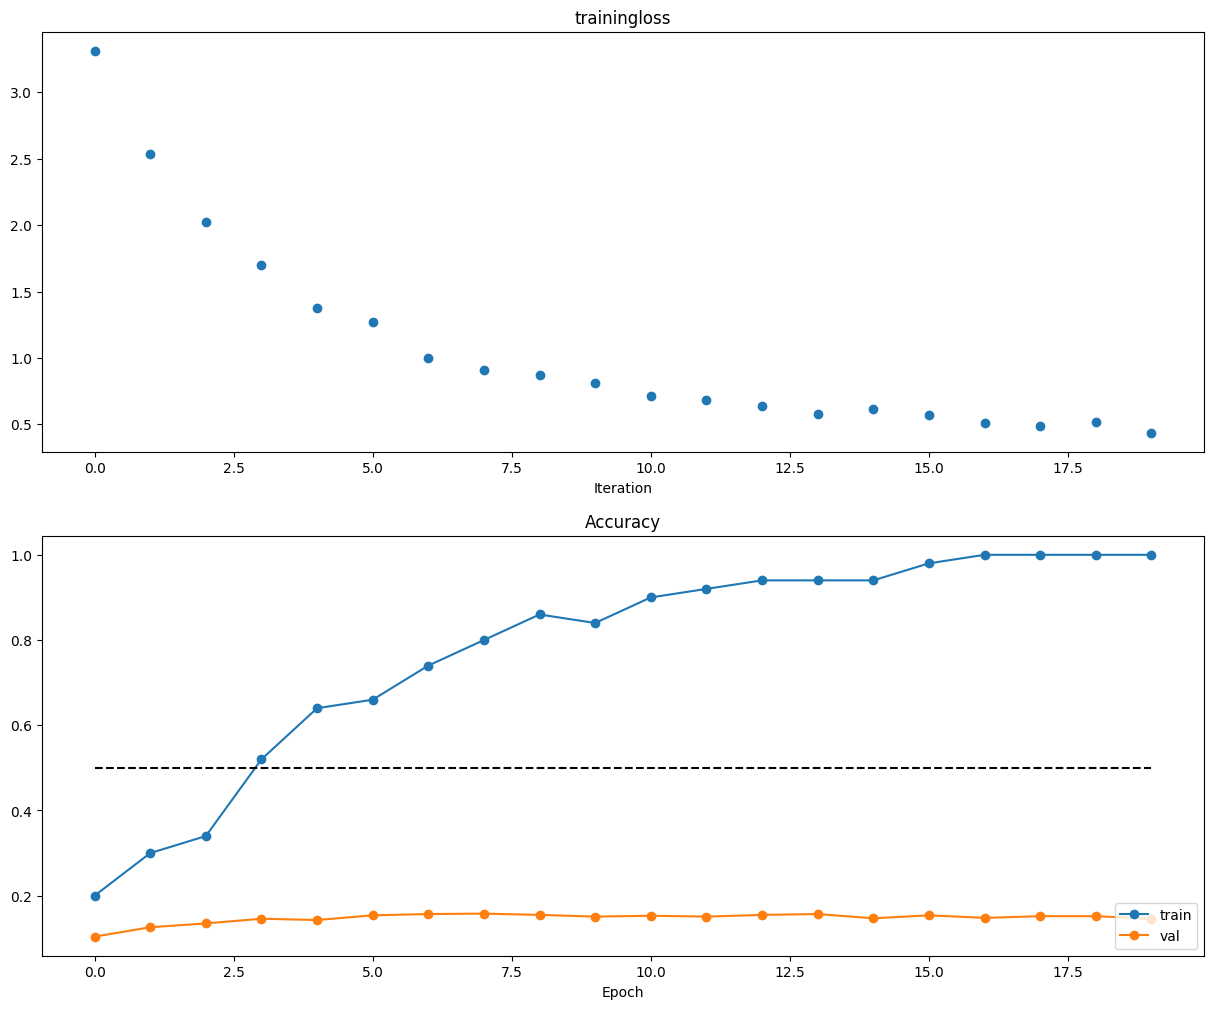
\includegraphics[scale = 0.32]{../nets/overfit_net/diagrams.png}}}  
    \end{figure}

  \item \textbf{Training a net}\\
    Architecture: 1 hidden layer with 100 hidden units.\\
    Hyperparameters: sdg update rulle, 5e-4 learning rate, 0.95 learning rate decay, 20 epochs, and a batch size of 100.
    \include*{../nets/train_net/info}
    
    \begin{figure}[!ht]
        \centering
        {{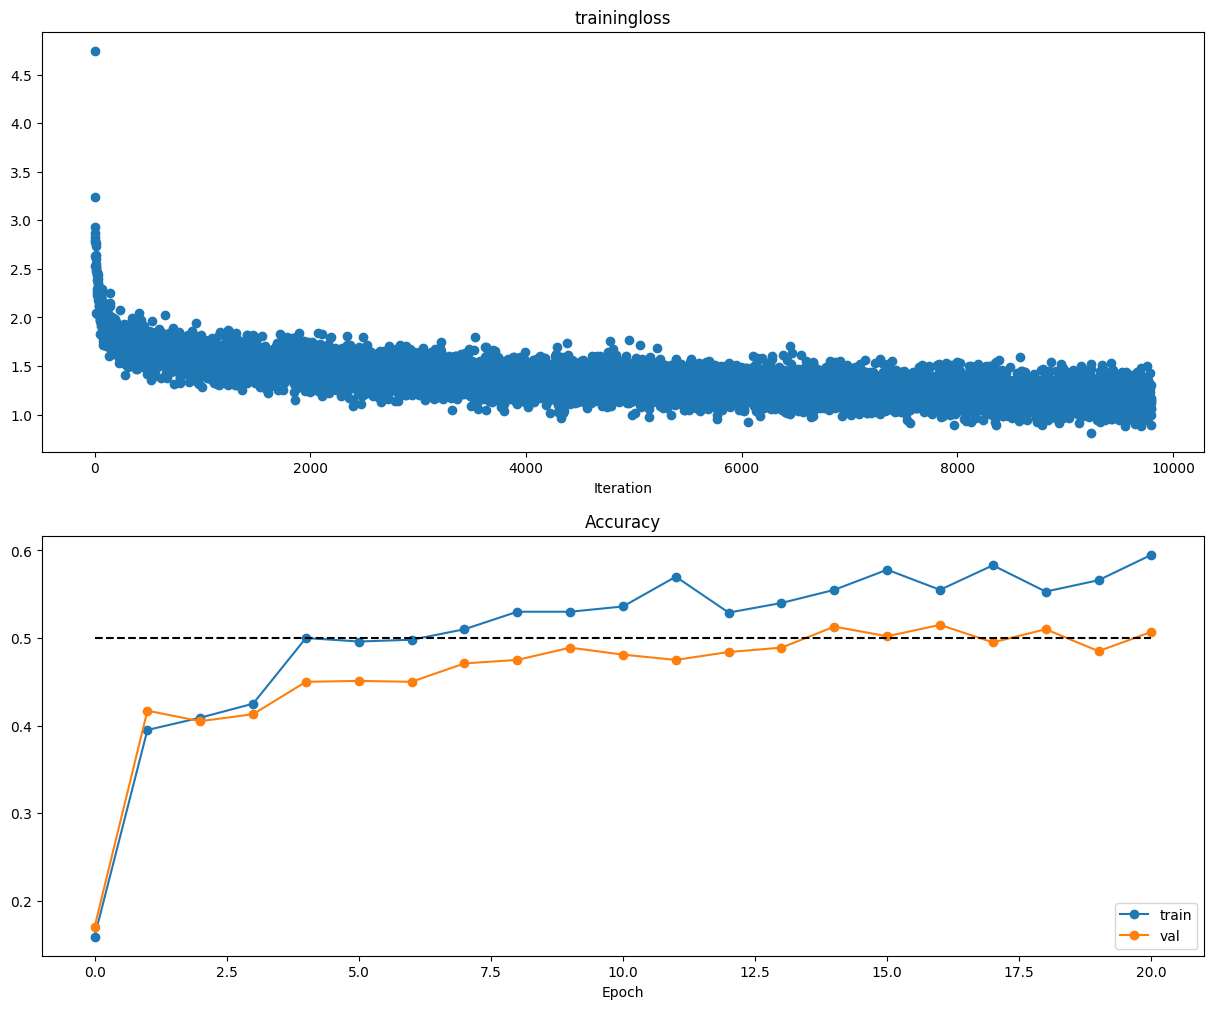
\includegraphics[scale = 0.32]{../nets/train_net/diagrams.png}}}  
    \end{figure}


\end{itemize}
